\documentclass[tikz,border=8pt]{standalone}
% Shared look for every TikZ diagram. Load with \input{../../tools/tikz-style.tex}
\usepackage[T1]{fontenc}
\usepackage{lmodern}
\renewcommand{\sfdefault}{lmr}  % diagrams use the same serif as the text
\usetikzlibrary{arrows.meta, positioning, shapes.geometric, calc, fit, backgrounds}
\definecolor{cblue}{HTML}{4C78A8}
\definecolor{corange}{HTML}{F58518}
\definecolor{cgreen}{HTML}{54A24B}
\definecolor{cred}{HTML}{E45756}
\definecolor{cpurple}{HTML}{B279A2}
\definecolor{cgrey}{HTML}{6B6B6B}
\tikzset{
  every picture/.style={font=\sffamily, line width=1.2pt},
  box/.style={draw=#1, fill=#1!12, rounded corners=4pt, align=center, inner sep=7pt, minimum height=1.1cm},
  box/.default=cgrey,
  arrow/.style={-{Stealth[length=3mm]}, draw=cgrey, line width=1.4pt},
  title/.style={font=\sffamily\bfseries\Large},
  note/.style={font=\sffamily\small, text=cgrey, align=center},
}
\AtBeginDocument{\hyphenpenalty=10000 \exhyphenpenalty=10000}

\begin{document}
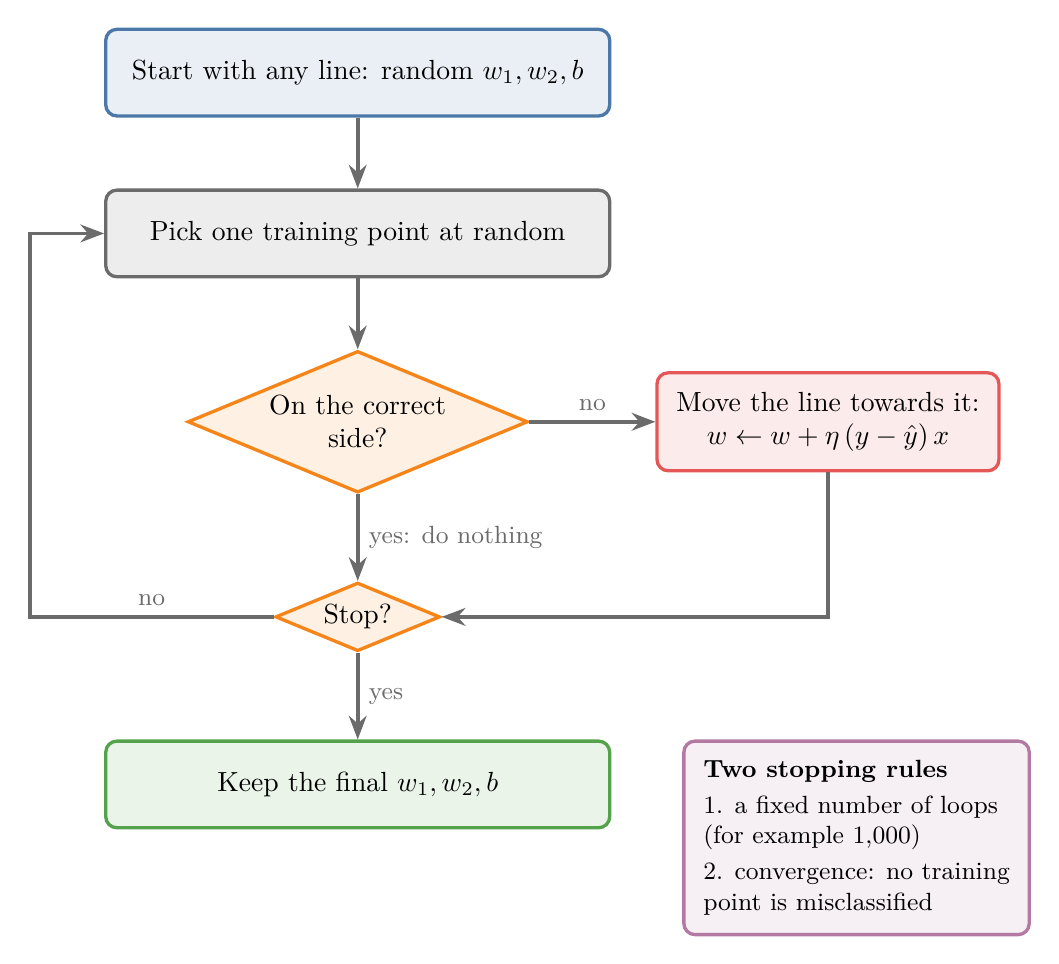
\begin{tikzpicture}[node distance=0.9cm]
  \tikzset{dec/.style={diamond, aspect=2.4, draw=corange, fill=corange!12, align=center, inner sep=2pt}}
  \node[box=cblue, minimum width=6.4cm] (init) {Start with any line: random $w_1, w_2, b$};
  \node[box=cgrey, minimum width=6.4cm, below=of init] (pick) {Pick one training point at random};
  \node[dec, below=of pick] (ok) {On the correct\\side?};
  \node[box=cred, minimum width=4.2cm, right=1.6cm of ok] (move) {Move the line towards it:\\$w \leftarrow w + \eta\,(y - \hat{y})\,x$};
  \node[dec, below=1.1cm of ok] (stop) {Stop?};
  \node[box=cgreen, minimum width=6.4cm, below=1.1cm of stop] (done) {Keep the final $w_1, w_2, b$};
  \draw[arrow] (init) -- (pick);
  \draw[arrow] (pick) -- (ok);
  \draw[arrow] (ok) -- node[right, note] {yes: do nothing} (stop);
  \draw[arrow] (ok) -- node[above, note] {no} (move);
  \draw[arrow] (move) |- (stop);
  \draw[arrow] (stop) -- node[right, note] {yes} (done);
  \draw[arrow] (stop.west) -- node[above, note] {no} ++(-3.1,0) |- (pick.west);
  \node[box=cpurple, align=left, anchor=north west, font=\sffamily\small] at ([xshift=0.9cm]done.north east) {\textbf{Two stopping rules}\\[2pt]
    1. a fixed number of loops\\(for example 1,000)\\[2pt]
    2. convergence: no training\\point is misclassified};
\end{tikzpicture}
\end{document}
